\documentclass[12pt,letterpaper]{article}
\usepackage[utf8]{inputenc}
\usepackage[total={18cm,21cm},top=2cm, left=2cm]{geometry} 
\usepackage{amsmath,amssymb,amsfonts,latexsym} 
\usepackage{graphicx} %gràficos y figuras
\usepackage{caption}
\usepackage{dsfont}
\usepackage{multicol}
\usepackage{color, xcolor}
\usepackage{hyperref}
\usepackage{float}
\definecolor{amarilloclaro}{RGB}{238,243,144}
\definecolor{azulclaro}{RGB}{210,243,243}
%\pagestyle{empty} %Elimina la numeración de las páginas
\parskip=0.5cm %Genera un espacio de 0.5cm entre los párrafos
\parindent=0mm %Elimina la sangría.
\renewcommand{\tablename}{Tabla}
\renewcommand{\figurename}{Figura}
\renewcommand{\refname}{Bibliografía}
\renewcommand{\abstractname}{Resumen}
%\spanishdecimal{.}
%nuevos comandos
\newcommand{\R}{\mathds{R}}
\newcommand{\sen}{\text{sen}}
\newcommand{\limite}[2] { \lim_{ #1 \rightarrow #2}}
\newcommand{\abs}[1]{\left| #1 \right|}
\newcommand{\norma}[1]{\left\| #1 \right\|}
\newcommand{\raiz}[3]{\sqrt{{#1}^2+{#2}^2+{#3}^2}}
%%
%Paquete Tikz
\usepackage{tikz}
\usepackage{pgfplots}
\pgfplotsset{compat=1.8}
\tikzset{flechaizq/.style={<-,>=latex}} 
\tikzset{flechader/.style={->,>=latex}}
\tikzset{flechadoble/.style={<->,>=latex}}
\tikzset{punteada/.style={line width=2, dash pattern = on 6pt off 3pt}}
\tikzset{continua/.style={line width=1, flechadoble}}
\tikzset{conector/.style={line width=2, flechadoble, dashed}}
\usetikzlibrary{shapes}
\usetikzlibrary{positioning}
\usetikzlibrary{intersections}
%%
\title{Métodos numéricos para resolver EDO}
\author{Jackeline, Luis Eduardo, David, Daniel, Over and Milton}

\date{}

\begin{document}
\maketitle
\begin{abstract}
 Aqui se escribe un resumen del trabajo  
\end{abstract}

\section{Ecuaciones diferenciales ordinarias}
Redactar teoría preliminar sobre EDO \cite[pp. 43]{librozill}

\section{Métodos numéricos para resolver EDO}
Redactar teoría sobre métodos numéricos de EDO.  A continuación vamos a referenciar una ecuación
\begin{equation}\label{ecug}
    x=\frac{-b\pm\sqrt{b^2-4ac}}{2a}
\end{equation}
La ecuación \eqref{ecug} es la solución a la ecuación cuadrátrica $ax^2+bx+c=0$.

\section{Códigos de programación en Python}
Este es un ejemplo para incrustar una imagen, referenciada como fig01. En la Figura \ref{fig01} se muestra
\begin{figure}[H]
    \centering
    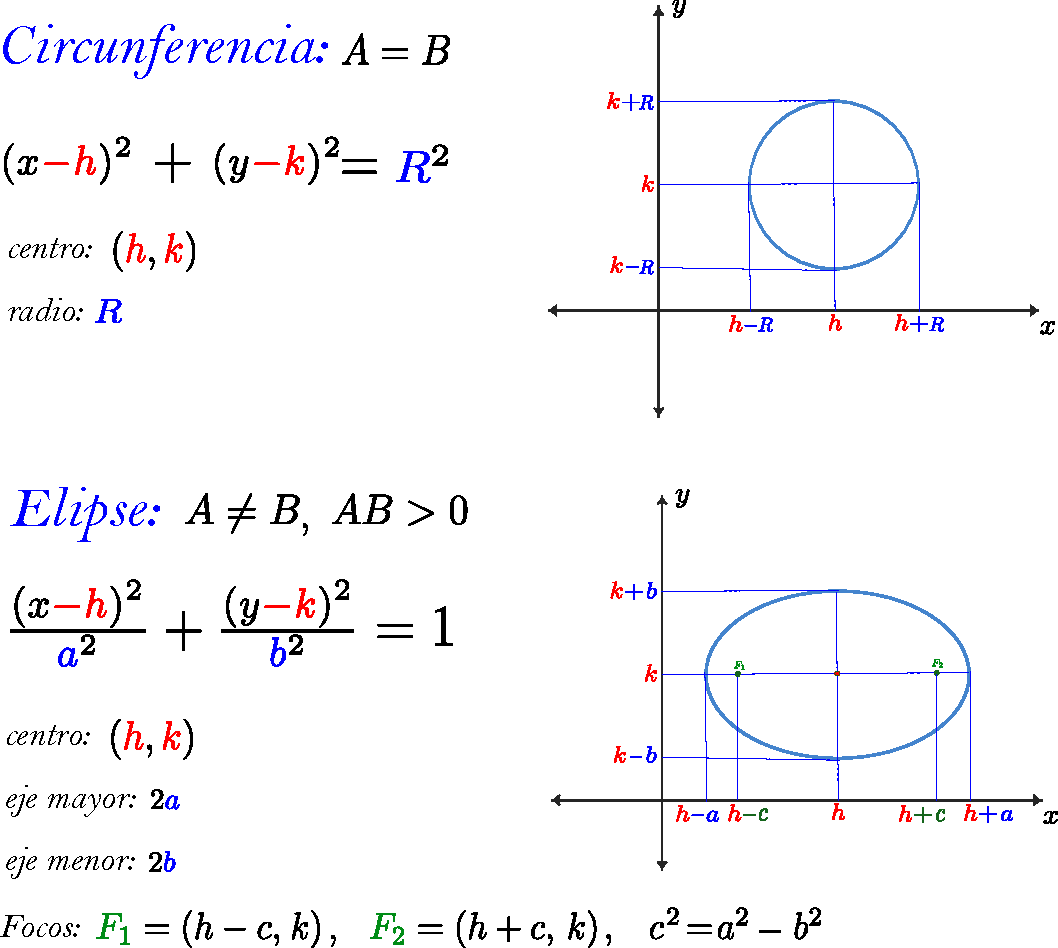
\includegraphics[scale=0.5]{images/elipse.pdf}
    \caption{Esta es una elipse}
    \label{fig01}
\end{figure}

Así se pone la bibliografia:
\bibliographystyle{unsrt}
\bibliography{referecias.bib}

\end{document}